% Adapted from Atanasio Rubio Gil's https://gitlab.com/Groctel/aqademia/-/blob/main/demo/demo_aqademia.tex

\documentclass[10pt, a4paper]{aqademic}

% Language and input encoding

\usepackage[spanish]{babel}

% Document settings

\usepackage[type=CC, modifier=by-nc-sa, version=4.0]{doclicense}
\usepackage{graphicx}
	\graphicspath{{img/}}
\usepackage{multirow}
\usepackage{adjustbox}
\usepackage{float}

\author{Daniel Pedrosa Montes}
\title{Arquitectura y Computación de Altas Prestaciones}

% Document composition

\begin{document}

\AqMaketitle[%
	cover    = identidad_ugr,
    subtitle = Manejo de MPI,
    url      = https://github.com/moshidev,
    date     = marzo del 2023 
]

\tableofcontents

\chapter{Resolución de los ejercicios propuestos.}
    Para las ejecuciones en nuestro ordenador local utilizamos \texttt{clang 14.0} sin flags
    adicionales de compilación además de los necesarios y para las ejecuciones en \texttt{atcgrid.ugr.es}
    utilizamos \texttt{gcc 9.2.0}.

    \section{Cálculo del producto escalar.}

Partimos del ejemplo 4 del primer seminario para implementar un programa
que nos permita realizar el cálculo del producto escalar. Para ello seguimos
los siguientes pasos, comprobando en cada uno de ellos que todo funciona según esperamos,
para diferente número de tareas y para diferente tamaño.

\begin{enumerate}
    \item Aisla el código cuya función es realizar la sumatoria de un vector en una función llamada `job`.
    \item Haz que el proceso MASTER participe en el cálculo, dividiendo la carga de trabajo entre todos los procesos.
    \item Haz que la recepción de los resultados de los workers se reciba de forma asíncrona, de forma que el MASTER pueda ir trabajando a la vez sin que esto suponga que los workers tengan que esperar a que termine este.
    \item Aisla el código del MASTER que se comunica con los workers en una función `scalarProduct`.
    \item Modifica la función job, worker y la que acabamos de crear de forma que haga el producto escalar.
\end{enumerate}

El ejecutable resultante tiene la misma interfaz que la del ejemplo 4.
Si, por ejemplo, decidimos un tamaño de 5 realizará la multiplicación $(0,1,2,3,4) \cdot (0,1,2,3,4)$.
Entendemos que la entrada de datos personalizados se escapa de los objetivos de la entrega.

Para compilar y ejecutar el ejercicio utilizamos \texttt{make run}.

    \pagebreak
    \section{Paralelización de un algoritmo de procesamiento digital de imágenes.}

    \pagebreak
    \section{Cálculo del Índice de Jaccard.}

Conociendo la intersección de los dos conjuntos podemos conocer este índice.
La mejor forma que encontramos para calcular la intersección de dos conjuntos
es la de utilizar un \textit{hashset}. Escogemos la implementación \textit{khash}.

Paralelizamos la carga de los datos en dos hebras, una por conjunto. De no ser así
ocurrirían condiciones de carrera al no ser la implementación escogida \textit{thread-safe}.

Una vez tenemos los dos conjuntos en memoria, paralelizamos el tamaño de la intersección
entre tantas hebras como queramos. Podemos hacer esto porque la lectura no modifica la
estructura de datos.

Ejecutamos con \texttt{make run}.

\subsection{Trabajo futuro.}

Podríamos paralelizar la carga de datos si permitiésemos que la estructura de datos fuese
reentrante. Para ello tal vez podríamos encontrar una solución que usase un cerrojo de espera
ocupada por cada \textit{bucket} junto a un \textit{mutex} que sincronizase el redimensionado
de la estructura de datos cuando fuese necesario (similar al problema de los lectores-escritores).
    
    \appendix
    \chapter{Fusión de bucles en el cálculo de Pi mediante distintos métodos.}
        Podemos identificar que ambos algoritmos utilizan un mismo número de pasos.
Como la localidad espacial no entra en juego para ninguno de estos podemos
acelerar la ejecución fusionando ambos bucles en uno. Modificamos el código,
ejecutamos las pruebas sobre \texttt{atcgrid} y obtenemos los resultados que
mostramos en la figura A.1.

\begin{figure}[H]
    \centering
    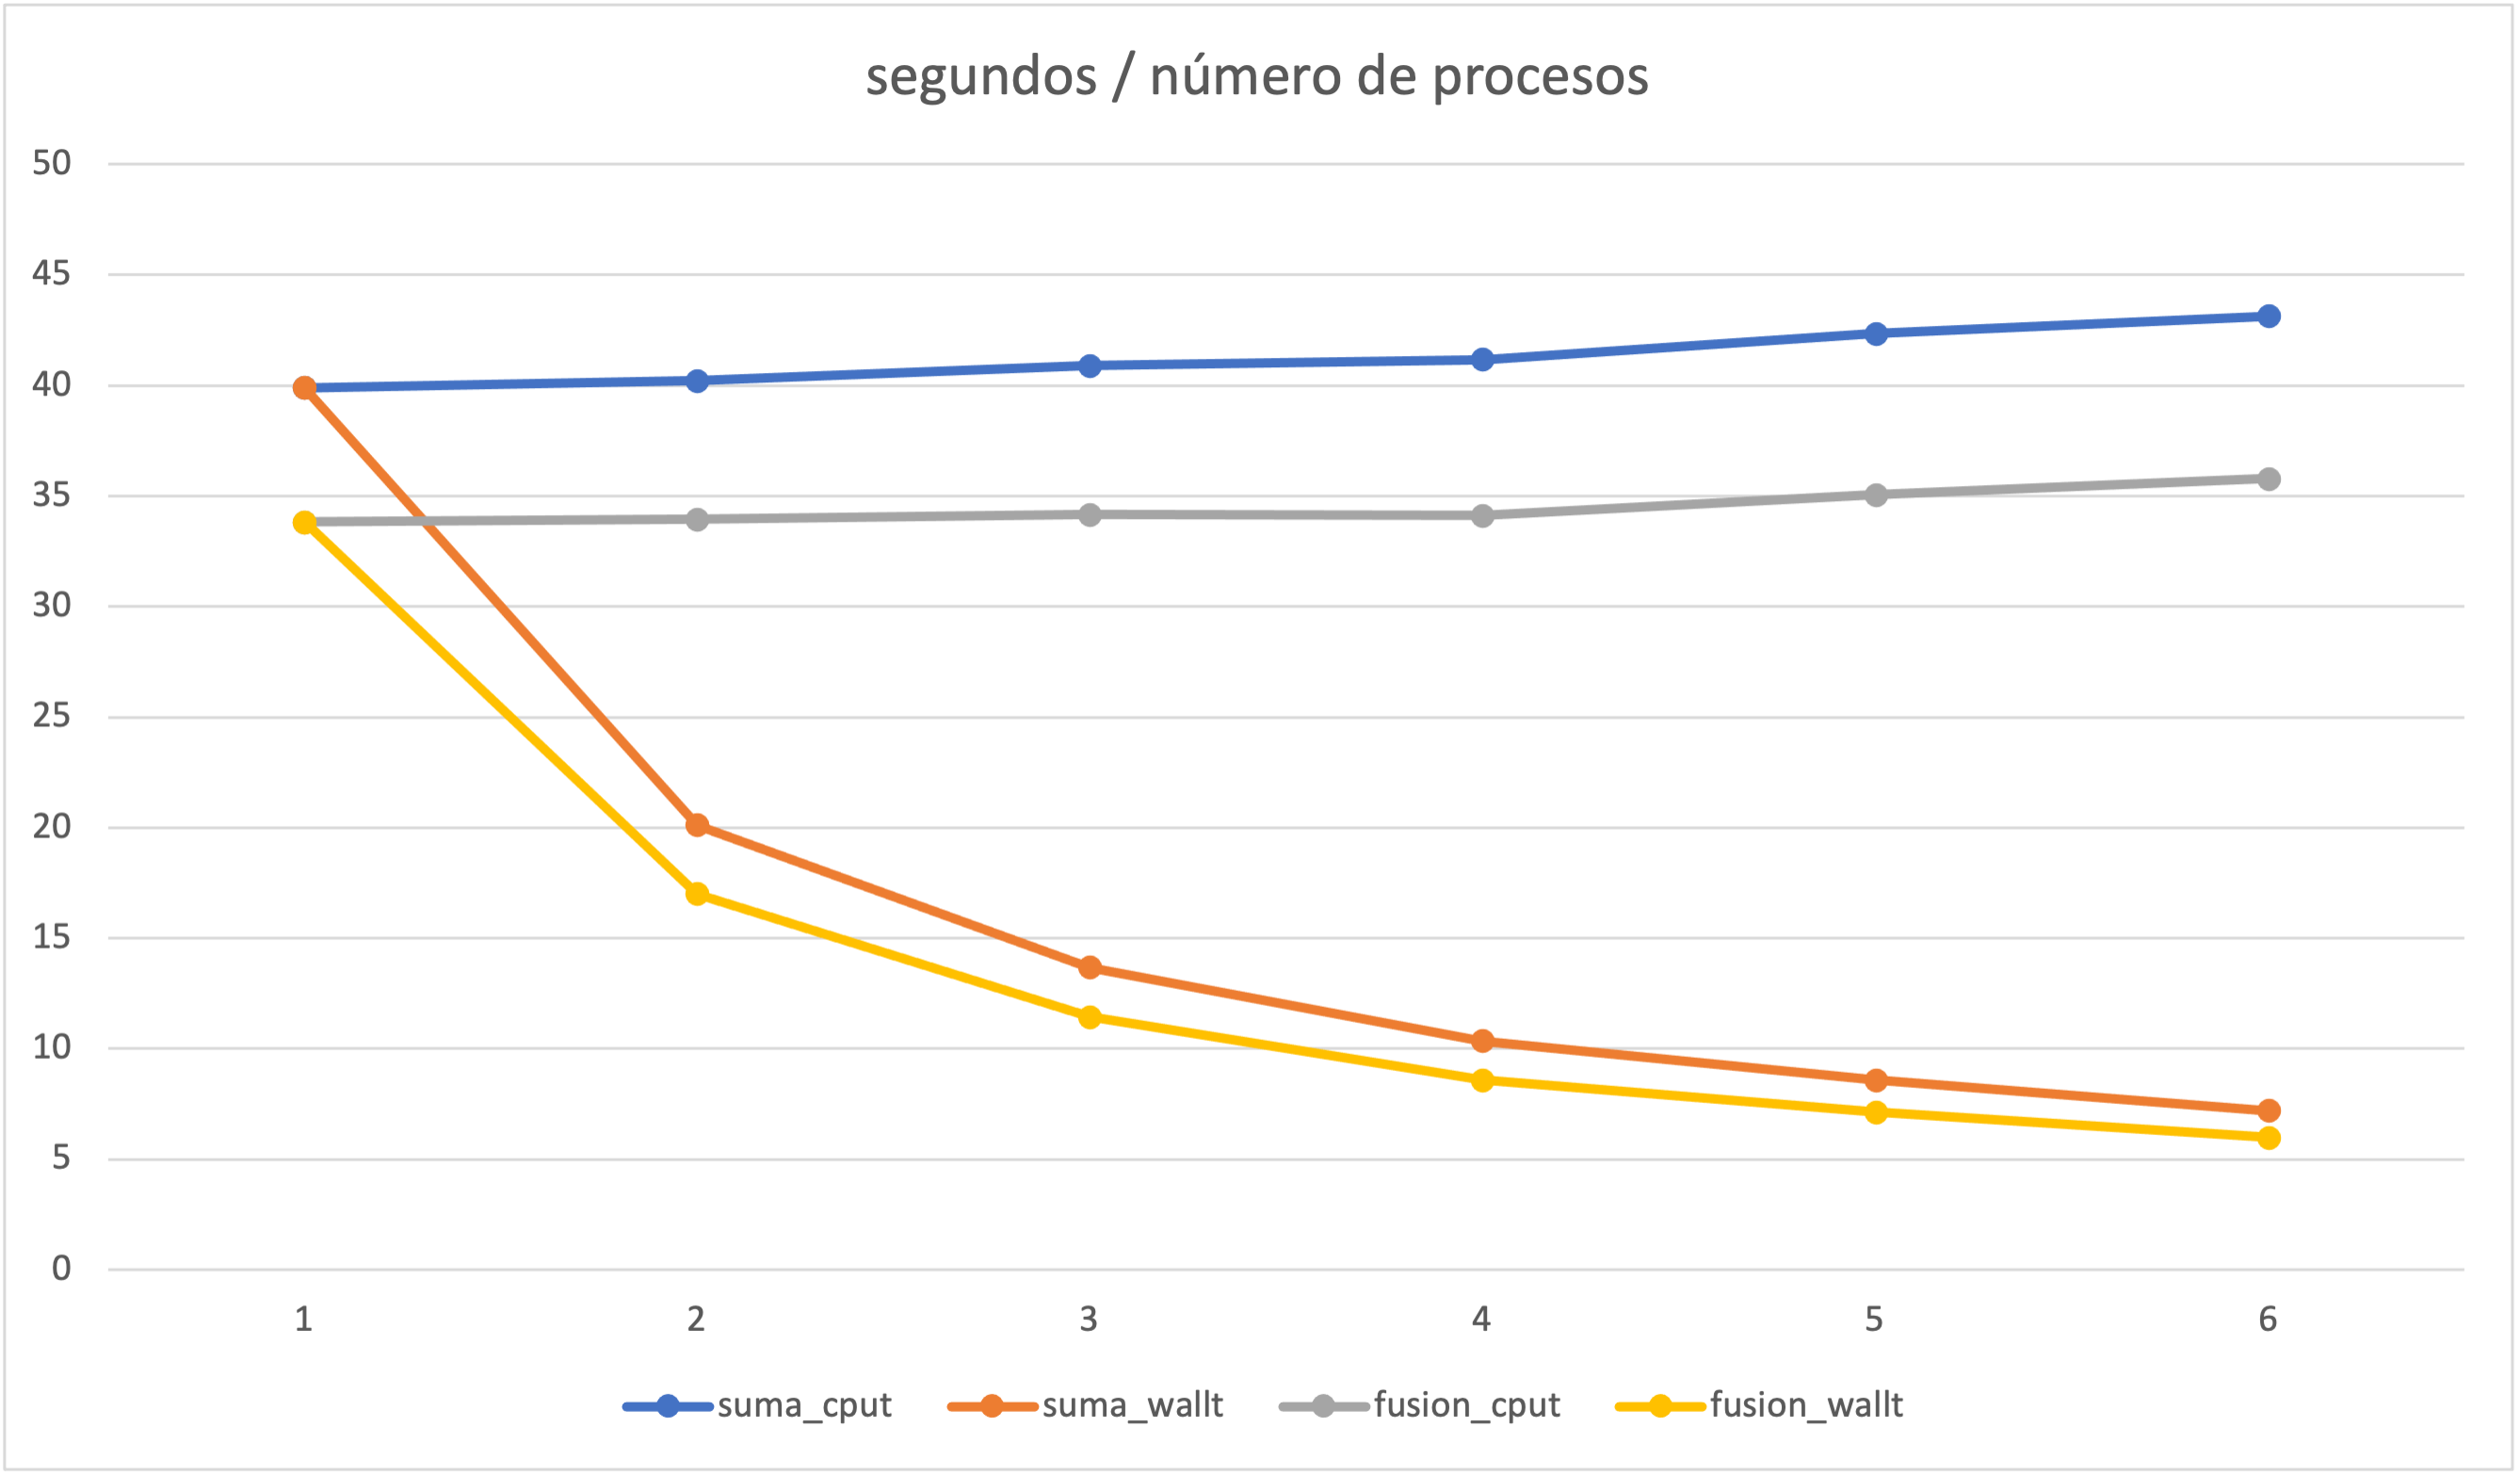
\includegraphics[width=16cm]{ap.png}
    \caption{Relación segundos / número de procesos. Observamos cómo los tiempos de ejecución para
    el algoritmo en que fusionamos ambos algoritmos son menores que la suma de los dos algoritmos ejecutándose
    por separado. Esto se debe a que se divide entre dos el tiempo que el procesador gasta controlando el bucle
    \texttt{for}.}
\end{figure}
    
\bibliographystyle{plain}
\bibliography{references}

\end{document}
